\section{Intrinsically Photosensitive Retinal Ganglion Cells (ipRGCs)}

\textit{Recent reviews by \citet{spitschan_melanopsin_2019}, \citet{do_melanopsin_2019},\citet{graham_melanopsin-expressing_2016} and \citet{lucas_melanopsin_2015} provide authoritative overviews of this rapidly progressing research area. This section shall focus on the subgroup of \glspl{ipRGC} called `M1' \glspl{ipRGC}, since these are the most populous and best understood; for details regarding the other subgroups of \glspl{ipRGC} see \citet{ecker_melanopsin-expressing_2010}.}

\bigskip

Retinal rod and cone cells (of three types, l/m/s) are well established as the primary receptors for human vision, and their connections and properties are relatively well understood. Two modes of vision originate from the retina, one of which is associated with image formation and the other which is considered to be \gls{NIF}, and which influences systems such as circadian rhythm entrainment, pupillary reflex and melatonin release. It was originally thought that rods and cones were the sole inputs to both of these modes of vision \citep{hankins_melanopsin_2008}.

\Glspl{RGC} combine signals from groups of cones and rods and relay these signals via the optic nerve to the lateral geniculate nucleus, which in turn processes and relays them further to the cortex for additional processing, allowing for classical vision of objects, movement and colour. \Glspl{ipRGC} are a sub-class of \glspl{RGC}, which in addition to combining and relaying signals exhibit some intrinsic photosensitivity of their own. 

This intrinsic photosenstivity was only confirmed recently relative to our knowledge of other retinal cell types \citep{qiu_induction_2005}, following a search for a retinal cell type or combination of cell types which would fit the spectral sensitivity properties found to influence entrainment of the circadian rhythm in humans and other animals \citep{brainard_human_2001,brainard_action_2001}, which was dissimilar to all of the spectral sensitivities of the cell classes known at the time.

Additionally, it was found that animals and humans with no functioning rods or cones were still able to have a correctly functioning circadian system \citep{freedman_regulation_1999,zaidi_short-wavelength_2007}, further suggesting that that the circadian rhythm was influenced by a novel receptor with a distinct photoreceptor. It is now believed to be these cells which provide input to the \gls{NIF} pathway.

\Glspl{ipRGC} were found to express a photopigment fitting such attributes, named melanopsin. The spectral sensitivity of melanopsin peaks around 480nm \citep{qiu_induction_2005,hankins_primary_2002,dacey_melanopsin-expressing_2005,peirson_melanopsin_2006,bailes_human_2013} which places it between the s-cone (cyanolabe photopsin) and rod cell (rhodopic rhodopsin) spectral sensitivities, see Figure \ref{fig:specsens}. In humans, pre-receptoral filtering leads to a functional peak sensitivity of closer to 490nm \citep{cie_cie_2015-1}. 

\begin{figure}[htbp]
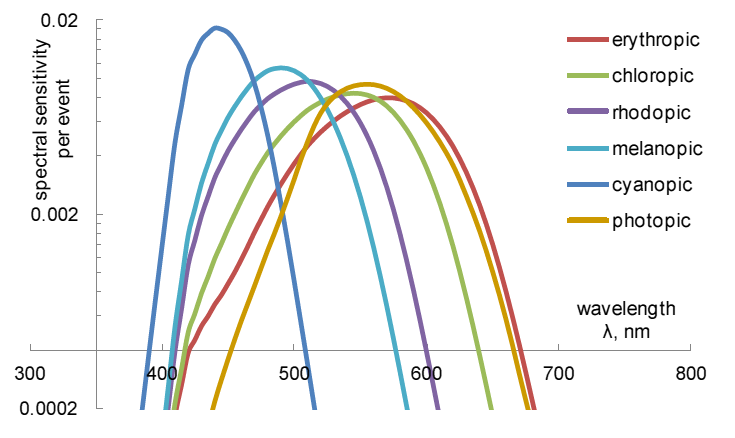
\includegraphics[max width=\textwidth, center]{figs/LitRev/ciemel.png}
\caption{Reproduced from \gls{CIE} TN 003:2015 \citep{cie_cie_2015-1}. \textit{``Spectral sensitivity curves of the five human photopigments to irradiance at the outer surface of the eye of the standard observer and photopic spectral efficiency, normalized to equal area.''}}
\label{fig:specsens}
\end{figure}

Exogenously expressed mouse melanopsin has been shown to be tristable \citep{emanuel_melanopsin_2015,matsuyama_photochemical_2012-1}, that is: existing in one of three possible states. A photon interaction converts melanopsin in one of these states to another, with two of the states being electrically silent (not providing a signal) and one being signal-producing. Notably, these different states have slightly different spectral sensitivities, and thus exposure to specific wavelengths biases the population distribution in different ways, as shown in Figure \ref{fig:melssf}.

\begin{figure}[htbp]
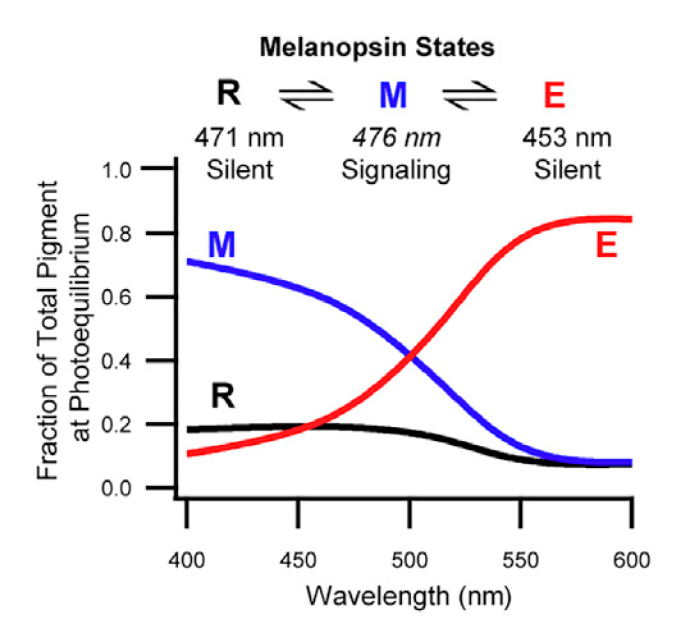
\includegraphics[max width=\textwidth, center]{figs/LitRev/melstates.png}
\caption{Reproduced from \citet{do_melanopsin_2019} (Fig 5D in original source). \textit{``[M]ouse melanopsin is understood to have three states (R, M, and E). The peak spectral sensitivities of R and E are determined from the electrophysiological responses of M1s. Spectrophotometric measurements of purified melanopsin yielded similar values (467 and 446 nm, respectively) and gave information for M (476 nm; [\citet{matsuyama_photochemical_2012-1}]). Bottom, the distribution of melanopsin states as a function of wavelength, estimated from a model based on values from purified melanopsin.''}}
\label{fig:melssf}
\end{figure}

Human melanopsin appears to be bistable (of two states), and there is uncertainty regarding whether this bistability has physiological consequences \citep{cie_cie_2015-1,mure_melanopsin_2009,rollag_does_2008,wada_color_2018,mure_melanopsin-dependent_2007,mawad_absence_2008,koyanagi_cephalochordate_2005,emanuel_melanopsin_2015}. It has been shown in other organisms that colour opponency from a single opsin is possible \citep{wada_color_2018}.

\Glspl{ipRGC} form a sparse mesh across the retina, each covering roughly 10$^{\circ}$ of visual angle \citep{ecker_melanopsin-expressing_2010}; discounting input from other cell types, they operate at a much lower resolution than as would be required for spatial vision of the type we are accustomed to. 

They also operate much more slowly than other cell types, taking several seconds to respond, but are able to sustain a response in contrast to other retinal cell types which are able to respond quickly but only for short periods (See Figure \ref{fig:melspeed} and \citet[p.210]{do_melanopsin_2019} for a summary).

\begin{figure}[htbp]
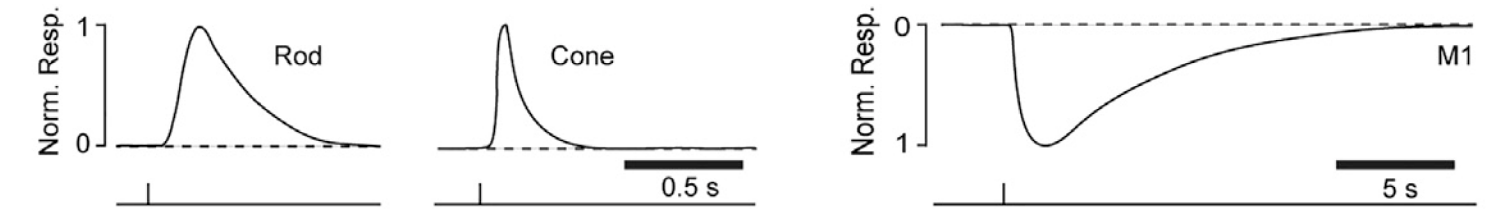
\includegraphics[max width=\textwidth, center]{figs/LitRev/melspeed.png}
\caption{Reproduced from \citet{do_melanopsin_2019} (Fig 5B in original source). \textit{``Dim-flash responses of outer photoreceptors and M1s (normalized photocurrent, having the same waveform as the single-photon response). Note the 10-fold
longer time base for the M1. The dashed line indicates the baseline current and the timing of the flash is shown below the curves, which are traced from
electrophysiological recordings (\citet{emanuel_biophysical_2017,field_nonlinear_2002,nikonov_physiological_2006}).''}}
\label{fig:melspeed}
\end{figure}

\Glspl{ipRGC} vary greatly in the range of light intensities that they are sensitive, are unimodal (stop responding above a certain threshold), and as a population their sensitivity spans a large range of lights levels \citep{do_melanopsin_2019}. It has been proposed that these properties \glspl{ipRGC} would allow an observer to efficiently sense a level of absolute irradiance \citep{brown_melanopsin_2010,milner_population_2017} (restricted to the wavelengths which ipRGCs and their inputs are sensitive to). 

\subsection{Synaptic Input}

In addition to their intrinsic photosensitivity, \glspl{ipRGC} exhibit extrinsic photosensitivity, taking inputs from rod and cone pathways in a similar fashion to regular \glspl{RGC}. Synaptic input is provided by amacrine and bipolar cells (See \citet{belenky_melanopsin_2003} and Figures \ref{fig:lucas} and \ref{fig:do}). 

\begin{figure}[htbp]
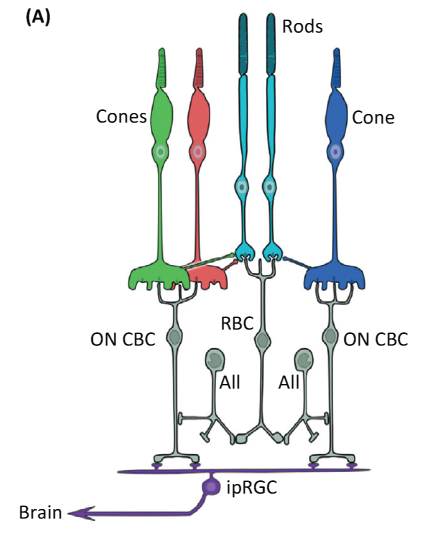
\includegraphics[max width=\textwidth, center]{figs/LitRev/lucas.png}
\caption{Reproduced from \citet{lucas_measuring_2014} (Figure 1A in origial source). \textit{``Schematic of the relevant retinal circuitry in humans. Non-image-forming responses originate in the retina and have been attributed to a particular class of retinal ganglion cell (ipRGC). ipRGCs are directly photosensitive owing to expression of melanopsin, which allows them to respond to light even when isolated from the rest of the retina. In situ they are connected to the outer retinal rod and cone photoreceptors via the conventional retinal circuitry. The details of their intraretinal connections are not completely understood and probably vary between different subtypes. Shown here are major connections with on cone bipolar cells (on CBCs) connecting them to cone and, via amacrine cells (AII) and rod bipolar cells (RBC), rod photoreceptors. As a consequence, the firing pattern of ipRGCs can be influenced by both intrinsic melanopsin photoreception and extrinsic signals originating in rods and each of the spectrally distinct cone classes (shown in red, green, and blue).''}}
\label{fig:lucas}
\end{figure}

\begin{figure}[htbp]
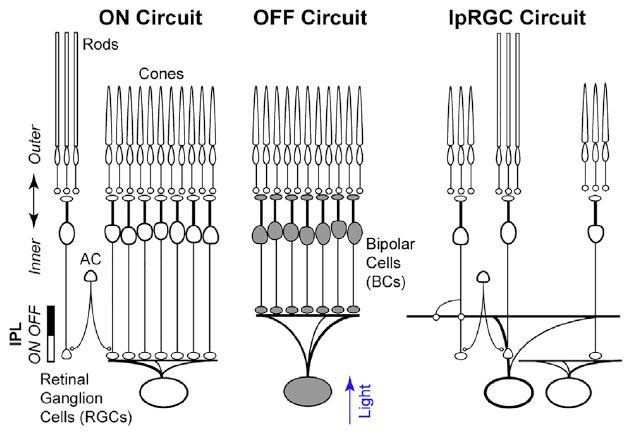
\includegraphics[max width=\textwidth, center]{figs/LitRev/do.png}
\caption{Reproduced from \citet{do_melanopsin_2019} (Fig 1A in original source). \textit{``A highly simplified schematic of the retina in cross-section, oriented with the inner aspect (nearer the center of the eye) down. The outer photoreceptors (i.e., rods/cones) drive bipolar cells (BCs). In the inner plexiform layer (IPL), BCs synapse with retinal ganglion cells (RGCs). Left: ON circuitry. Rods (top) drive rod BCs, whose signals pass through amacrine cells (ACs) to cone BCs. In the inner IPL, ON cone BCs convey signals to ON RGCs. ON RGCs show greater depolarization when light intensity increases. Center, OFF circuitry. In the outer IPL, OFF cone BCs provide synaptic input to OFF RGCs. OFF RGCs show greater depolarization when light intensity decreases. Right: a sample of circuits for outer- and inner-stratifying ipRGCs, which are both ON. ON cone BCs make ectopic synapses with the former and conventional synapses with the latter. Rod pathways also drive ipRGCs. IpRGCs make chemical and electrical synapses with ACs (not shown).''}}
\label{fig:do}
\end{figure}

Inputs evoke ON responses, despite originating from both the ON and OFF layers of the inner plexiform layer (see Figure \ref{fig:do}). \citet{graham_melanopsin-expressing_2016} describe the processes which allow this to occur: 

\begin{itquote}{}
ON bipolar cells use two unconventional strategies to release glutamate onto the dendrites of SCN-projecting mouse ipRGCs in the “OFF” sublamina. Some ON bipolar cells’ axons extend lateral protrusions that contain synaptic vesicles [...], whereas others possess en passant (in passing) synaptic vesicles within their axonal shafts [\citet{dumitrescu_ectopic_2009}]. Distally stratifying ipRGCs are also present in rabbit, marmoset and macaque retinas, and they likewise receive unconventional ON bipolar input in the “OFF” sublamina [...] [\citet{hoshi_inputs_2009}, \citet{grunert_bipolar_2011}].
\end{itquote}.

Signals from rods and cones retain their traditional time courses; \glspl{ipRGC} are not inherently sluggish, rather the melanopic inputs to \glspl{ipRGC} are. This can be seen in Figure \ref{fig:wong}, where standard outputs of an \gls{ipRGC} are shown on the left, and outputs with rod/cone driven synaptic inputs blocked are shown on the right. The response is shown to be relatively instantaneous for the cell with intact inputs, but lagging by several seconds for the cell relying on melanoptic activation alone.

\begin{figure}[htbp]
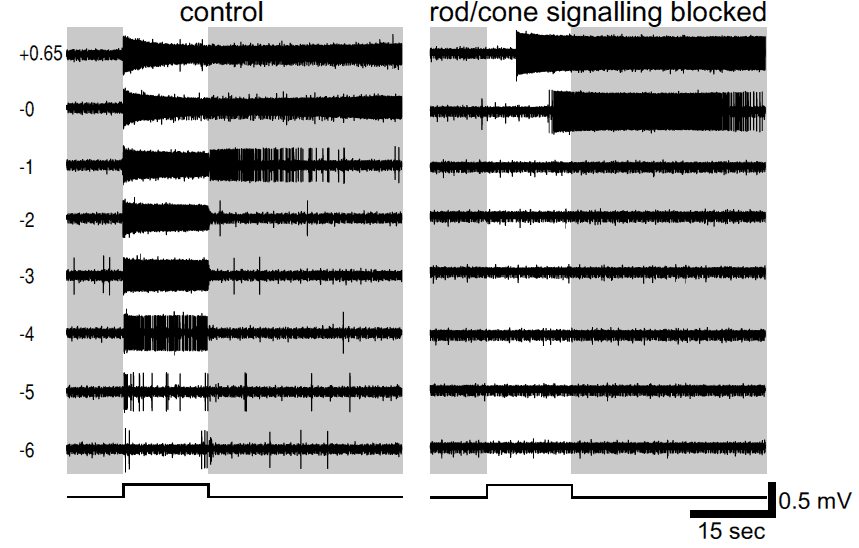
\includegraphics[max width=\textwidth, center]{figs/LitRev/wong.png}
\caption{Reproduced from \citet{wong_synaptic_2007} (Fig 4 in original source). \textit{``Multi-electrode array (MEA) recordings of synaptically mediated light responses in ipRGCs. Extracellular recordings comparing spike responses of an ipRGC to light of various intensities with rod/cone-driven synaptic inputs left intact (left) or blocked (right). Log stimulus attenuation is indicated to the left. Note that all responses to weaker stimuli (-2 log attenuation and dimmer) and short-latency responses to brighter ones (-1 to +0.65 log I) were dependent on synaptic transmission, presumably because they reflect rod and/or cone influence on the recorded cell. Note also that intensities sufficient to recruit the intrinsic response (-0 and +0.65 log I; right) evoke responses with substantial poststimulus persistence, a well-established feature of melanopsin-dependent light responses.''}}
\label{fig:wong}
\end{figure}

There also evidence for \glspl{ipRGC} having intraretinal retrograde synaptic output (\citet{zhang_intraretinal_2008,zhang_melanopsin_2012}, summarised by \citet{graham_melanopsin-expressing_2016}), via a subpopulation of dopaminergic amacrine cells. This type of signalling could provide a feedback loop which modifies signals before they have left the retina.

\clearpage

\subsection{Projection}

\glspl{ipRGC} have been shown to innervate `dozens of brain areas' \citep{do_melanopsin_2019}, with M1s principally innervating \gls{NIF} areas, but with some activation of areas traditionally thought of as image-forming. There appear to be meaningful differences between the different sub-types of \gls{ipRGC} in this respect, with different sub-types (denoted M1-6, distinguished by their retinal morphology) showing distinct activation pathways. 

A summary of these projections is shown in Figure \ref{fig:projection}. From this figure it can be seen that there are still many potential projections which have not been investigated (``Each blue dot indicates the approximate density of innervation by its size, a white dot indicates undetectable innervation, and lack of a dot indicates an absence of information.''). However, it can clearly be seen that outputs are extensive and varied.

\begin{figure}[htbp]
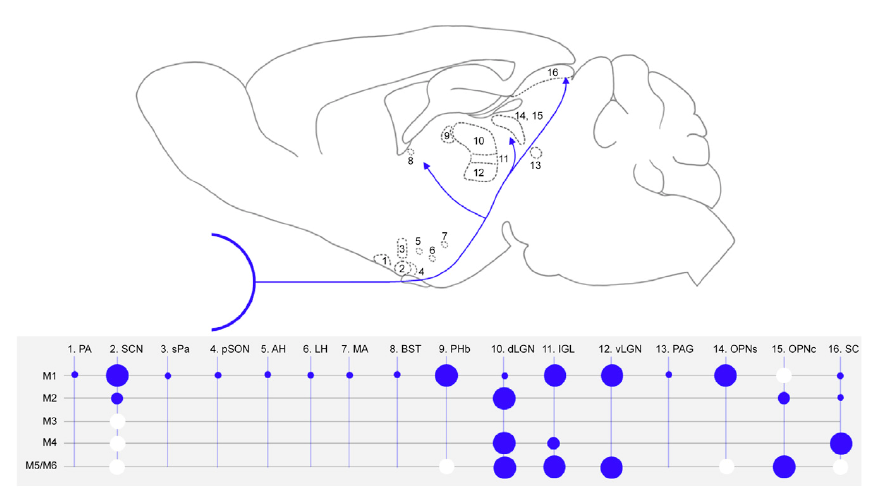
\includegraphics[max width=\textwidth, center]{figs/LitRev/projection.png}
\caption{Reproduced from \citet{do_melanopsin_2019} (Fig 3 in original source). \textit{``Major Brain Targets of Mouse IpRGCs. A sample of ipRGC brain targets is depicted in a quasi-sagittal schematic of the mouse brain. Below is a plot of innervation densities across ipRGC types, drawn after Berson and colleagues (\citet{quattrochi_m6_2019}) and incorporating additional information (\citet{ecker_melanopsin-expressing_2010}; \citet{hattar_central_2006}; \citet{huang_visual_2019}; \citet{morin_retinofugal_2014}; \citet{zhao_photoresponse_2014}). Each blue dot indicates the approximate density of innervation by its size, a white dot indicates undetectable innervation, and lack of a dot indicates an absence of information. M5s and M6s are pooled because their projections were examined together for technical reasons. AH, anterior hypothalamus; BST, bed nucleus of the stria terminalis; dLGN, dorsal lateral geniculate nucleus; IGL, intergeniculate leaflet; LH, lateral hypothalamus; MA, medial amygdala; OPN, olivary pretectal nucleus (with shell, s, and core, c, regions); PA, preoptic area, which includes the VLPO (ventrolateral preoptic area); PAG, periaqueductal gray; PHb, perihabenular zone; pSON, peri-supraoptic nucleus; SC, superior colliculus; SCN, suprachiasmatic nucleus; sPa, subparaventricular zone; and vLGN, ventral lateral geniculate nucleus.''}}
\label{fig:projection}
\end{figure}

\clearpage

\subsection{The roles of ipRGCs beyond circadian entrainment}
\label{sec:ipRGCbeyond}

In recent years there has been a number of publications examining the role of melanopsin outside of \gls{NIF} vision, challenging some of the assumptions about the abilities of signals originating from \glspl{ipRGC}.

A number of studies have found that the signals from ipRGCs are capable of encoding spatial structure \citep{ecker_melanopsin-expressing_2010, mouland_responses_2017, allen_melanopsin_2017, allen_form_2019, zhao_photoresponse_2014}\footnote{For commentary see \citet{spitschan_vision_2017} and \citet{sonoda_re-evaluating_2016}.}, and others have probed the influence upon brightness perception \citep{zele_cone_2018,brown_melanopsin-based_2012}

Additionally, several researchers have investigated whether \glspl{ipRGC} may play a role in chromatic vision \citep{cao_evidence_2018, spitschan_human_2017-1,zele_melanopsin_2018,horiguchi_human_2013,vincent_adaptation_2019,vincent_adaptation_2019-1}, using the silent substitution paradigm \citep{estevez_silent_1982,spitschan_method_2018}\footnote{Though see \citet{kamar_silent-substitution_2019}.}. These studies are summarised below.

\citet{spitschan_human_2017-1} found an fMRI response in primary visual cortex for each of four participants, in contradiction to an earlier study by the same group \citep{spitschan_human_2016}\footnote{``we now regard our prior study as not fully resolving the possibility that rapid modulation of the ipRGCs drives a cortical response'' \citep{spitschan_human_2017-1}}. Participants reported a visual percept which was ``unpleasant, blurry, minimal brightening that quickly faded''. There also seemed to be evidence of a chromatic perception: ``Many of the subjects described the melanopsin stimulus pulse as being colored. This was typically a yellow–orange appearance, although three subjects reported a greenish percept''.


\citet{cao_evidence_2018} found that ``changing melanopsin activation levels shifts the equilibrium point in the chromatic pathways'', though curiously the effect was only present for the L/(L+M) pathway. This is shown in Figure \ref{fig:cao}. The authors conclude that melanopsin activation affects the parvocellular pathway to the extent that \gls{ipRGC} activation could be thought of as ``additive to the M-cone signal opposing the L-cone signal in the PC pathway [i.e., L - (M + I)] (where ``I'' for melanopsin activation in ipRGCs) to signal greenness and/or blueness''. The authors note that this corresponds to an earlier result from one of the same authors \citep{barrionuevo_contributions_2014} where such a contribution set was proposed. However, the earlier result includes rod contributions, and the specific pathway which they must be referring to is only the 5th component accounting for $<0.01\%$ of the variance. Meanwhile, no evidence is found for the 2nd component from that same analysis (labelled as konioncellular, representing $1.56\%$ of variance), which they also proposed would have a considerable melanopic contribution contribution. They neglect to mention this in the later paper.

\begin{figure}[htbp]
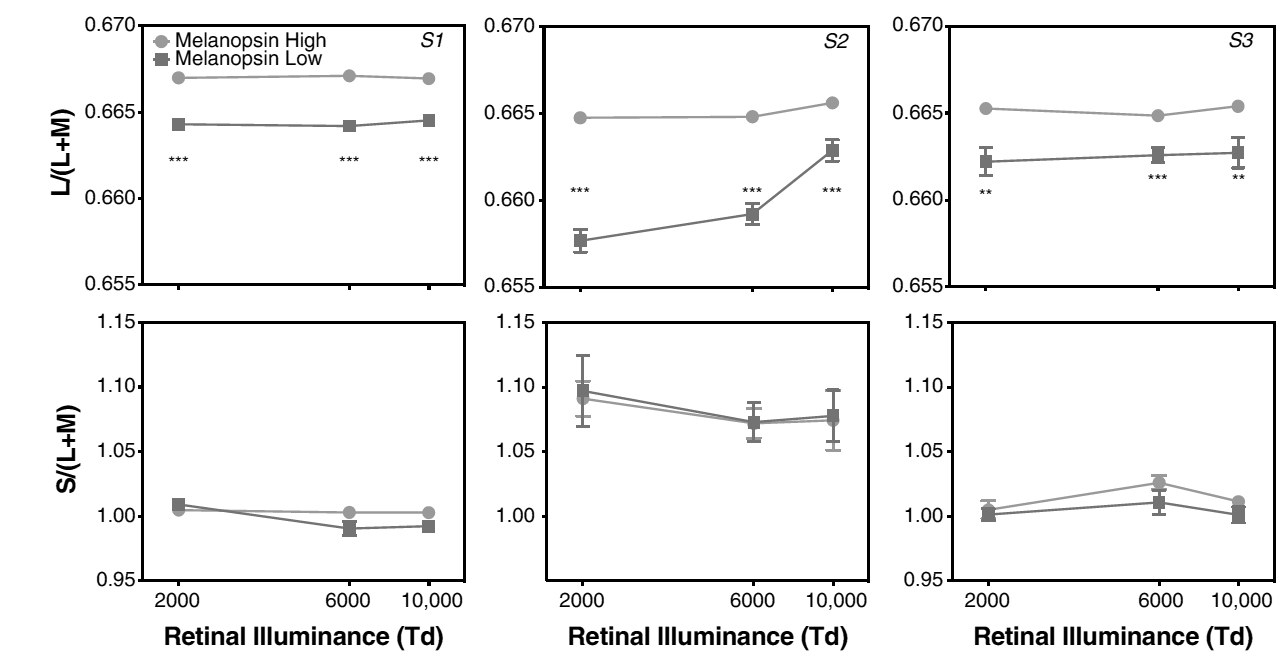
\includegraphics[max width=\textwidth, center]{figs/LitRev/cao.png}
\caption{Reproduced from \citet{cao_evidence_2018} (Figure 1 in original source). \textit{``Unique white $l$ (top) and $s$ (bottom) values (mean $\pm$ sem)
as a function of retinal illuminance for three observers. **$p < 0.01$;
***$p < 0.001$ from t-tests.''}}
\label{fig:cao}
\end{figure}

\citet{zele_melanopsin_2018} found evidence that ``putative melanopsin-mediated image-forming vision corresponds to an opponent S-OFF L+M-ON response property, with an average temporal resolution up to approximately 5 Hz, and $>$10x higher thresholds than red-green colour vision''. The key figure from this study is reproduced in Figure \ref{fig:zele}. This figure shows the perceptual matches to melanopic contrasts in terms of equivalent cone contrasts, for four observers, under three different conditions. For each observer, and for each condition, it can be seen that a melanopic contrast can be matched by an L+M increment and a S/(L+M) decrement.

\begin{figure}[htbp]
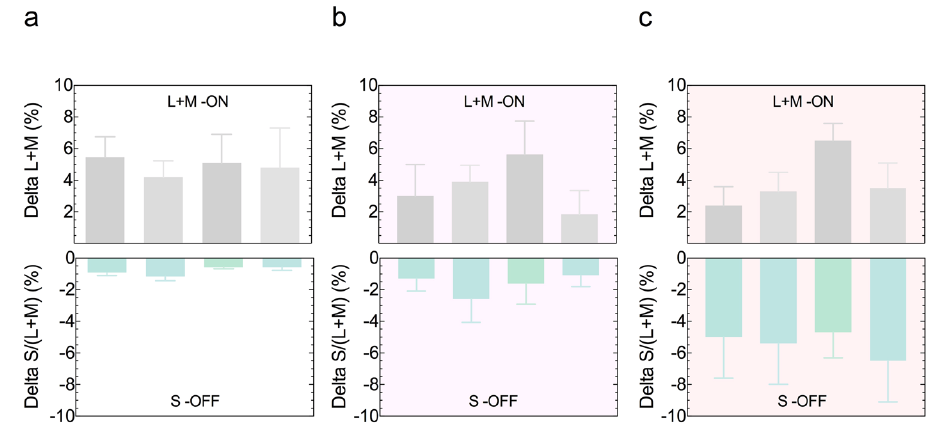
\includegraphics[max width=\textwidth, center]{figs/LitRev/zele.png}
\caption{Reproduced from \citet{zele_melanopsin_2018}. \textit{``Melanopsin photoreception is analogous to an increment in cone luminance [L + M] and a decrement in S-cone excitation [S/(L + M)] with white (a), yellowish-pink (b) and orange adapting stimulus fields (c). [...] Data in each panel are for four participants (mean $\pm$ SEM) measured at 2000 photopic Td.''}}
\label{fig:zele}
\end{figure}

This appears to be a perfect contradiction to the results of \citet{cao_evidence_2018}: \citet{cao_evidence_2018} found a parvocellular response and no koniocellular response whilst \citet{zele_melanopsin_2018} found a koniocellular response\footnote{Albeit inverted: S-OFF L+M-ON, rather than the traditional S-ON L+M-OFF \citep{hendry_koniocellular_2000}.} and no parvocellular response\footnote{Though the matching values for this pathway aren't actually reported. One assumes they did not exhibit a trend and/or fell below some meaningful threshold.}. However, attention should be paid to the distinctions in experimental goals and procedures. \citet{cao_evidence_2018} probe the long term adaptive effects of differing levels of melanopic activation upon white settings, whereas \citet{zele_melanopsin_2019} probe the equivalent appearance of melanopsin in terms of cone-based percepts. It is possible that this distinction is the root of the inconsistency.

Very recent results from \citet{vincent_adaptation_2019,vincent_adaptation_2019-1} report that, contrary to expectations (based on the work of \citet{allen_melanopsin-driven_2014}), ``sensitivity to flicker directed at the cones was not altered by adaptation to a steady field of substantially higher melanopic content''. This appears to rule out the hypothesis that melanopsin activation alters gain (aka adaptation) at an early retinal level for cone-based signals.

The final study which needs note here is the work of \citet{horiguchi_human_2013}. In this study the authors find that ``[i]n the periphery, at high photopic levels, human sensitivity is not accurately explained by absorptions in only three types of cone photopigments [requiring a fourth]''. This work focuses on discrimination thresholds rather than attempting to understand a direct perceptual correlate to melanopic stimulation.

Though these results are exciting, there are a number of methodological and theoretical areas which require development. The standard methodology used in these experiments is that of `silent substitution' \citep{estevez_silent_1982,kamar_silent-substitution_2019,spitschan_method_2018} where careful tuning of the spectrum is used (see the topic of `metameric blacks' \citep{vienot_verriest_2014,cohen_metameric_1982,vienot_domain_2012,vienot_dimensionality_2015}) to generate signals which are only visible to the chosen receptor-type in theory, in this case melanopsin-expressing \glspl{ipRGC}. 

However, due to variability in observer spectral sensitivities, and limits on the level of stimulus control, it is likely that there will be a small amount of unintended stimulation of non-target cell groups. \citet{spitschan_selective_2015} refer to this as `splatter' (``the expected amount of contrast on nominally silenced photoreceptor classes for a given modulation around a given background''). A suggested control condition is to generate contrast for the nominally silenced cell groups at the level predicted from modelling.

A further concern: horizontal cell feedback can result in nominally silenced cone populations still producing an output. \citet{kamar_silent-substitution_2019} discussed this issue further.

\subsubsection{Value for colour constancy}

In this section I shall outline the reasoning which suggests to me that there might be value in a melanopic input for attaining colour constancy.

Existing colour constancy algorithms fundamentally rely on the ability of cone-receptor-based signals to calibrate cone-receptor-based signals. In this context, by \emph{calibrate} I mean  \emph{modify a raw signal in order to exclude unwanted signal, in order to improve the accuracy (and possibly also precision) of target signal measurement} where the \emph{unwanted signal} would be variation in illumination, and the target signal would be either the \gls{SRF} of a surface or some other identifier of the surface.

This general framework suffers from what I refer to as the issue of circularity in self-calibration\footnote{I suspect that this issue has been discussed in other fields but I have been unable to find such discussion as of yet.}. Generally calibration is performed by characterising a sensor through measurement of an object where the ground truth is known (and/or a measurement from a trusted secondary sensor has been made of this object), and adjusting the properties of the sensor (either at the measurement stage or by implementing a post-processing stage) such that a measurement of the known object results in the expected values. In the case outlined above (cone-receptor-based signals calibrating cone-receptor-based signals), there is no ground truth object, and no secondary sensor, and thus calibration in the traditional sense fundamentally cannot be performed.

If only relative signals are of importance (as opposed to absolute value measurements), then an uncalibrated system might satisfactory stability through the use of measurements taken over time or over space from a single sensor.

A melanopic signal could represent a secondary signal, and the properties of \glspl{ipRGC} seem to make them well-suited for making measurements where the ambient illumination is preferentially detected over transient \glspl{SRF}. Particular properties will be discussed below.

If one's goal was to design a sensor which measured the ambient illumination upon a scene (and was only minimally perturbed by surface reflectances) it might be wise to limit both the spatial and temporal resolution relative to sensors which may be best for measuring surfaces, since the lighting on a scene generally operates at spatial and temporal frequencies which are both lower than surface variation within a scene, particularly when the scene is not viewed from a static position but from a constantly changing vantage (such as is the case with human vision, where the observer is moving body, face direction, and gaze direction regularly). It would also be ideal if the secondary sensor was not strongly adaptive, as this would allow for a more concrete relationship between stimuli and response. As noted previously, \glspl{ipRGC} exhibit all of the above properties.

There are multiple sites at which a melanopsin-based calibration could occur. The synaptic connections to \glspl{ipRGC} from rods and cones could allow a melanopsin-dependent transform to be performed at the \gls{RGC} stage before signals are output. Alternatively, the intraretinal outputs from \glspl{ipRGC} could allow for modification of signals before reception by traditional \glspl{RGC}. Finally, calibration could occur at any higher post-retinal location assuming that melanopic and cone-based signals could be reconstructed at that point.





\clearpage


